\section{Mesh-Netz}
\label{sec:KonzeptionMeshNetz}
Für die Entwicklung eines Mesh-Netzes muss zunächst eine Topologie designt werden, die den Eigenschaften der Sensorknoten entsprechen. In das Netzwerk muss zu einem ein Sensorknoten eingebunden werden der extrem energiesparend ist, ein normaler Sensorknoten der über eine dauerhafte Stromversorgung verfügt und ein Gateway zum Internet. Jeder dieser Geräte hat unterschiedliche Anforderungen und teilweise auch verschiedene Betriebssysteme. 
\begin{figure}
	\centering
	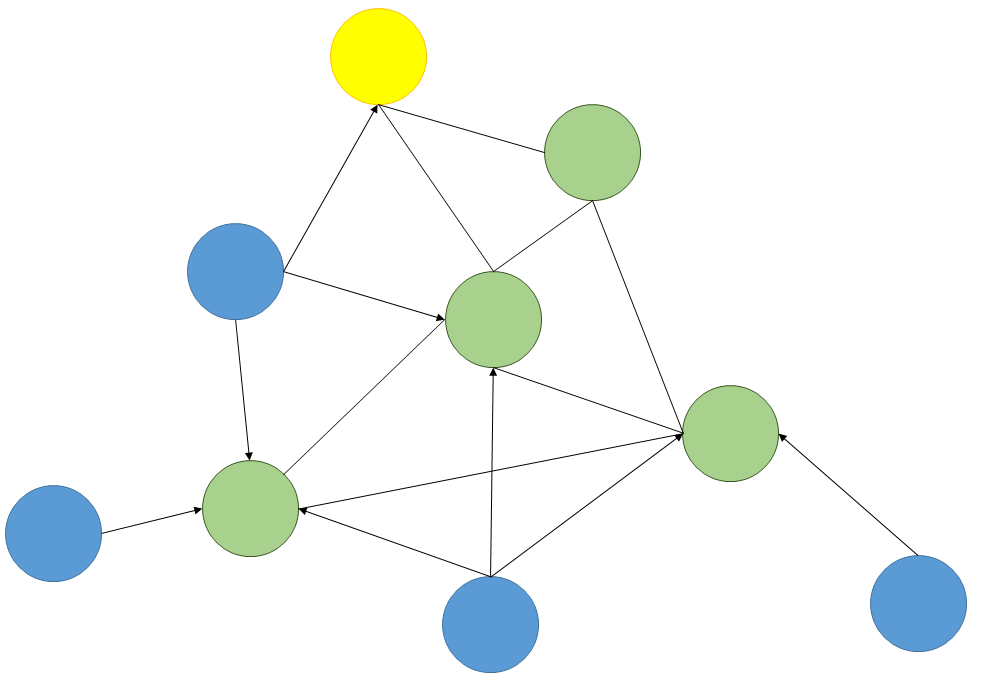
\includegraphics[width=0.6\textwidth]{bilder/konzeptionMeshTopologie}
	\caption[Topologie Mesh-Netz]{Topologie Mesh-Netz: blaue Knoten $\rightarrow$ energiesparende Sensorknoten, grüne Knoten $\rightarrow$ normale Sensorknoten und gelber Knoten $\rightarrow$ Gateway}
	\label{img:konzeptionTopologie}
\end{figure}

In der Konzeptionsphase wurden die Geräte in drei Gruppen unterteilt. Dies waren die normalen Sensorknoten, energiesparende Sensorknoten und ein Gateway zum Datenbankserver/Internet. In der Grafik \ref{img:konzeptionTopologie} ist die Topologie des Mesh-Netzes zu sehen.
\paragraph{Normaler Sensorknoten} Dieser Sensorknoten übernimmt neben der Messwerterfassung noch das Weiterleiten von Nachrichten im Netztwerk. Hierfür ist er mit einer dauerhaften Stromversorgung ausgestattet. Während der Sendephase des Sensorknotens kann dieser keine Nachrichten empfangen und weiterleiten. Wenn der Sensorknoten nicht in der Sendephase ist hört er die gesamte Zeit in das Netzwerk und wartet bis er eine Nachricht empfängt. Der genaue Ablauf wird im darauffolgenden Paragraphen genauer erläutert. Wie in den Grundlagen (\ref{sec:Mesh-Netz} Kapitel) erläutert ist, handelt es sich um einen aktiven Knoten, genauer um einen Mesh-Router. Mit diesen Geräten kann das Netz, bezüglich Reichweite, erweitert werden.
\paragraph{Energiesparender Sensorknoten} Beim energiesparenden Sensorknoten handelt es sich nur um einen Mesh-Client (siehe \ref{sec:Mesh-Netz} Kapitel). Das bedeutet, dass er ist ein passiver Knoten im Mesh-Netz ist. Dieser übernimmt keine Weiterleitungsaufgaben im Netzwerk. Nachdem der Sensorknoten seine Messwerte erfasst und gesendet hat geht dieser Knoten in einen Schlafmodus. Mit diesem Sensorknoten ist es nicht möglich die Reichweite des Netzwerks zu erhöhen. Dieser Knoten ist darauf angewiesen, dass entweder ein normaler Sensorknoten in der Nähe ist oder direkt das Gateway.
\paragraph{Gateway zum Internet} Beim der letzten Komponente des Mesh Netzes handelt es sich um das Gateway zum Internet. Dieses Modul übernimmt nur das Empfangen von Nachrichten. Das Gateway ist im permanenten Empfangsmodus und wartet auf das Eingehen neuer Nachrichten. Nachdem das Datenpaket enkodiert ist wird sichergestellt, dass diese Nachricht zum ersten Mal angekommen ist. Wenn die Nachricht zum ersten Mal erhalten wurde, wird der Messdatensatz dauerhaft gespeichert. 
\paragraph{Programmablaufplan Mesh-Algorithmus} Nachdem wir die einzelnen Geräte genauer beleuchtet haben wird in diesem Abschnitt auf den  selbst entwickelte Art von Mesh-Algorithmus eingegangen. In der Grafik \ref{img:PAPMeshAlgo} ist der Programmablaufplan bei einem normalen Sensorknoten zu sehen. Dieser beschreibt das Vorgehen, beginnend vom Empfang einer Nachricht bis zum Verwurf der Nachricht bzw. Weiterleiten der Nachricht. 

\begin{figure}
	\centering
	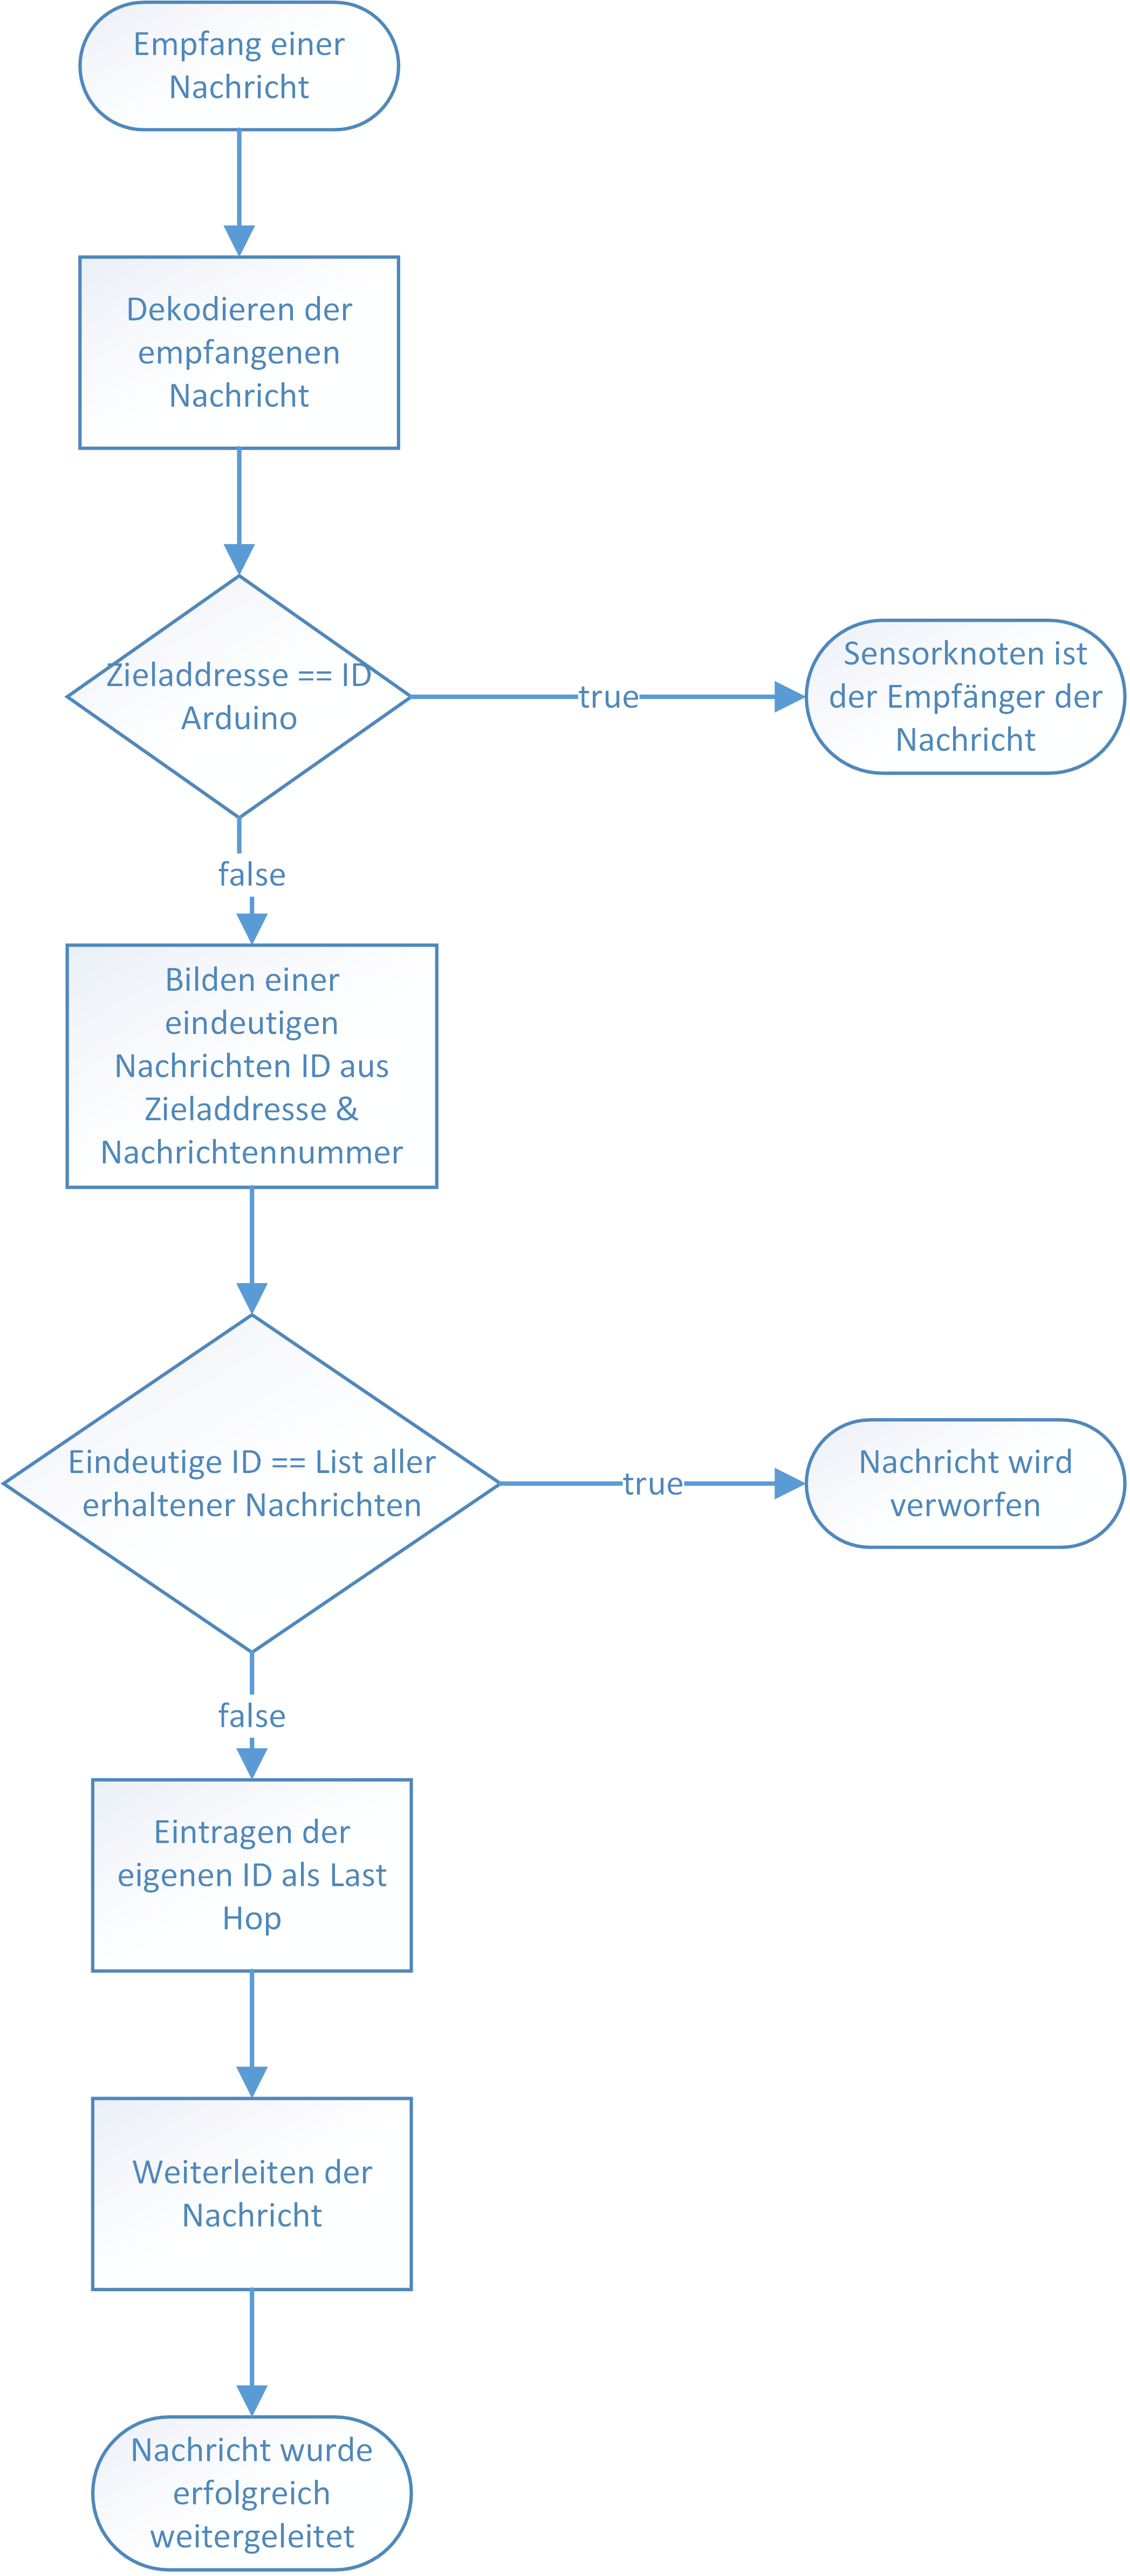
\includegraphics[width=0.6\textwidth]{bilder/PAPMesh.png}
	\caption{Programmablaufplan - Mesh- Algorithmus}
	\label{img:PAPMeshAlgo}
\end{figure}
